\documentclass[]{IEEEtran}
\usepackage{float}
\usepackage{multicol}
\usepackage[a4paper, margin=0.68in]{geometry}
\usepackage{color} %red, green, blue, yellow, cyan, magenta, black, white
\definecolor{mygreen}{RGB}{28,172,0} % color values Red, Green, Blue
\definecolor{mylilas}{RGB}{170,55,241}
\usepackage[siunitx]{circuitikz}
\usepackage{siunitx}
\usepackage{verbatim}
\usepackage{lscape}
\usepackage{listings}
\usepackage{courier}
\usepackage{gensymb}
\usepackage{amsmath,amsfonts,mathtools,amssymb}
%opening
\title{ECEN405 Lab 1}
\author{Keshav Raj 300418412\\Lab Partner: Tim Loretto}

\begin{document}
	\onecolumn
\lstset{language=Matlab,%
	%basicstyle=\color{red},
	breaklines=true,%
	morekeywords={matlab2tikz},
	keywordstyle=\color{blue},%
	morekeywords=[2]{1}, keywordstyle=[2]{\color{black}},
	identifierstyle=\color{black},%
	stringstyle=\color{mylilas},
	commentstyle=\color{mygreen},%
	showstringspaces=false,%without this there will be a symbol in the places where there is a space
	numbers=left,%
	numberstyle={\tiny \color{black}},% size of the numbers
	numbersep=9pt, % this defines how far the numbers are from the text
	emph=[1]{for,end,break},emphstyle=[1]\color{red}, %some words to emphasise
	%emph=[2]{word1,word2}, emphstyle=[2]{style},    
}
\maketitle
\markboth{Note}
{}

\begin{multicols}{2}
\section{Deliverables}
\subsection{1)}
\begin{equation*}
	\begin{split}
		30k&=\frac{10k}{32.8k(1k)C_1}\\
		30k&=\frac{10k}{32.8M\ C_1}\\
		\frac{1}{C_1}&=\frac{30k\cdot32.8M}{10k}\\
		C_1&=\frac{10k}{30k\cdot32.8M}\\
		C_1&=10.1626nF\\
		C_1&\approxeq10nF\\
		\end{split}
\end{equation*}
\subsection{2)}
In order to find the minimum frequency, $R_3$ needs to be minimized and $R_4$ needs to be maximized. By entering the formula into desmos and assigning $R_3$ to be the X axis and $R_4$ an adjustable slider, the entire range of frequencies can be investigated.
\begin{figure}[H]
	\centering
	\caption{Minimum frequency at $R_3=0\Omega$ and $R_4=100k\Omega$}
	\label{fig:screenshot001}
	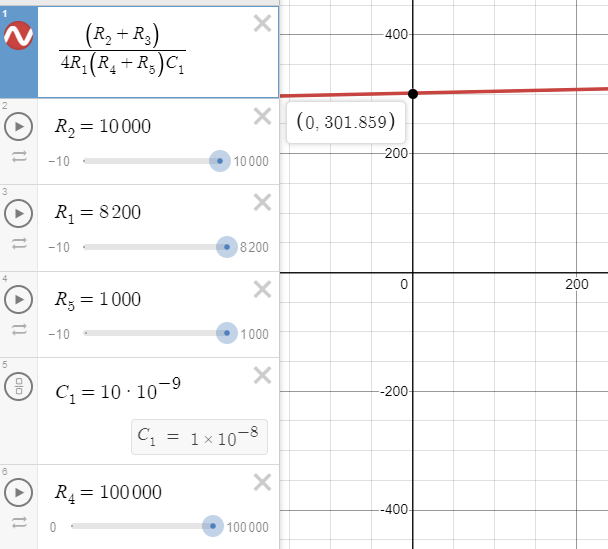
\includegraphics[width=1\linewidth]{screenshot001}
\end{figure}
\begin{figure}[H]
	\centering
	\caption{Maximum frequency when $R_3=1M\Omega$ and $R_4=0\Omega$}
	\label{fig:screenshot002}
	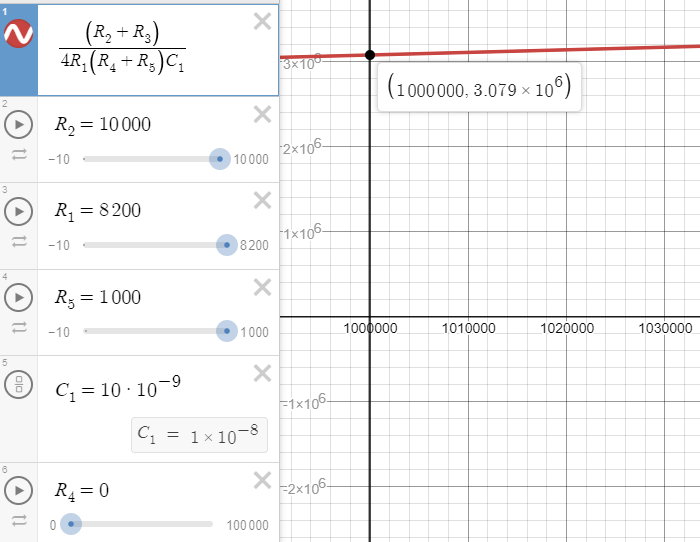
\includegraphics[width=1\linewidth]{screenshot002}
\end{figure}
These two figures show that the minimum frequency is 301Hz while the max is 3MHz.
\subsection{3)}

\end{multicols}
\begin{figure}[H]
	\centering
	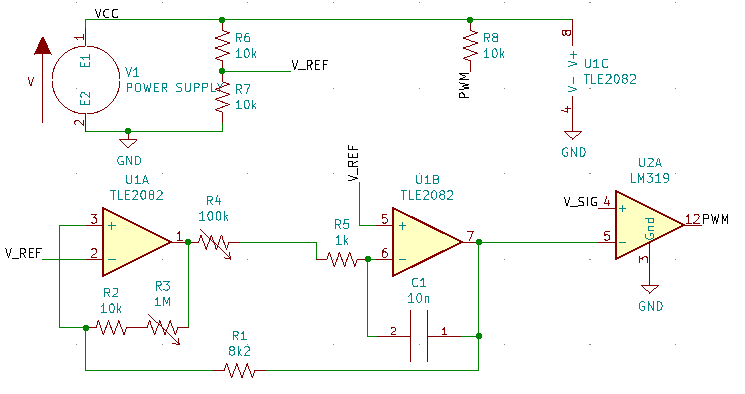
\includegraphics[width=1\linewidth]{screenshot003}
	\caption{Schematic of PWM Generator}
	\label{fig:screenshot003}
\end{figure}
\begin{multicols}{2}
	\subsection{4)}
	%TODO
	\subsection{5)}
	All op-amps have a drop off in gain with increasing frequency, eventually as the frequency gets so high, the op-amp's gain attenuates too much too be seen on the output. Also the frequency response of some of the components used such as the resistors and capacitors would prevent the realization of high frequency signals and would most likely just filter them out.
	\subsection{6)}
	Rather than having a single comparator, one can have two with the second one with its inputs swapped (input signal goes to inverting input and triangle wave goes to non-inverting input), this would allow a non-inverted and an inverted signal to be generated. Otherwise one could use a logic inverter to achieve the same.
\end{multicols}



\end{document}
